\documentclass[a4paper,11pt]{article}
%\usepackage[T1]{fontenc}

%\setlength{\textwidth}{20cm}
%\setlength{\marginparwidth}{0cm}
%\setlength{\voffset}{0cm}
\usepackage[utf8]{inputenc}
\usepackage[francais]{babel}
\usepackage{amsmath}
\usepackage{graphicx}
\usepackage{listings}
\usepackage{color}
%==== to fix locations of figures and tables
\usepackage{float}
\usepackage{placeins}

\lstset{
language=VHDL,
basicstyle=\small\sffamily,
numbers=left,
numberstyle=\tiny,
frame=tb,
columns=fullflexible,
showstringspaces=false
}
%\special{papersize=210mm,297mm}

\title{{\Huge Electronique numérique}\\Initiation à VHDL (2/3)\\Circuits séquentiels. Automates.\\ \color{red}{CORRECTIONS}}
%\title{TD1}
\date{}

\begin{document}
\maketitle

\boxed{Questions}


\boxed{CORRECTIONS}
Nous proposons ici plusieurs architectures pour le même calcul, en conservant une seule entité.
\paragraph{Architecture combinatoire}

\lstset{inputencoding=utf8}
\lstinputlisting[language=VHDL]{./code/ab_plus_cd_unsigned.vhd}

\paragraph{Autres architectures (séquentielle)}
\lstset{inputencoding=utf8}
\lstinputlisting[language=VHDL]{./code/ab_plus_cd_other_arch.vhd}

\paragraph{Banc de test}
\lstinputlisting[language=VHDL]{./code/ab_plus_cd_tb.vhd}
\begin{figure}
  \centering
  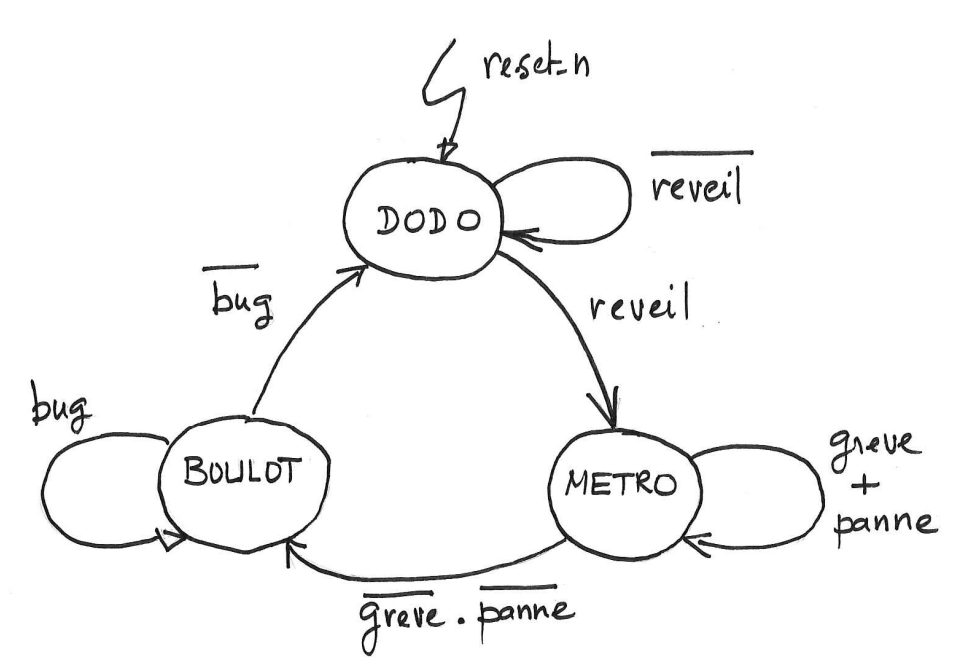
\includegraphics[width=8cm]{./iloveparis.png}
  \caption{Simulation associée au banc de test "ab\_plus\_cd\_tb.vhd"}
  \label{ab_plus_bc}
\end{figure}



\paragraph{Note complémentaire}
Le problème portait sur le codage des premières bascules D. Profitons en pour nous pencher sur un point tout autre...La traduction directe de l'équation donnée n'a
été rendue possible que par "chance". Par exemple, un codage identique, mais avec des opérandes non-signés n'aurait pas fonctionné comme attendu...
La dynamique des signaux est un sujet délicat. En général, il faut gérer explicitement ces "range", notamment à l'aide de la fonction "resize".
Nous rappelons ici les règles élémentaires \textbf{théorique} (hors VHDL) concernant la taille des opérandes, en nombre de bits, pour l'addition
et la multiplication de deux nombres $a$ et $b$, possédant chacun $n_a$ et $n_b$ bits.

% \begin{tabular}{|c|c|c|}
%   \hline
%   type de donnée & nombre de bits du résultat & exemple \\ \hline \hline
% $+_{unsigned}$ & $max(n_a,n_b)+1$ & $255+255=510$          i.e $[8]_u+[8]_u=[9]_u$ \\ \hline
% $*_{unsigned}$ & $n_a+n_b$        & $255*255=65025$        i.e $[8]_u*[8]_u=[16]_u$ \\ \hline
% $+_{signed}$   & $max(n_a,n_b)+1$ & $127+127=254$          i.e $[1+7]_s+[1+7]_s=[1+8]_s=[9]_s$ \\ \hline
% $*_{signed}$   & $n_a+n_b-1$      & $(-128)*(-128)=+16384$ i.e $[1+7]_s*[1+7]_s=[1+14]_s$ \\ \hline
% \end{tabular}

\begin{tabular}{|c|c|c|}
  \hline
  type de donnée & nombre théorique de bits & VHDL numeric\_std \\ \hline \hline
$+_{unsigned}$ & $max(n_a,n_b)+1$ & $max(n_a,n_b)$\\ \hline %OK
$*_{unsigned}$ & $n_a+n_b$        & $n_a+n_b$\\ \hline      %OK
$+_{signed}$   & $max(n_a,n_b)+1$ & $max(n_a,n_b)$\\ \hline %OK
$*_{signed}$   & $n_a+n_b$        & $n_a+n_b$\\ \hline      %
\end{tabular}

Par défaut, les fonctions du package numeric\_std ne rendent pas un résultat exact, mais \textbf{tronqué} en ce qui concerne
les additions.

\begin{lstlisting}
function "+" (L,R: UNSIGNED ) return UNSIGNED;
    -- Result subtype: UNSIGNED(MAX(L'LENGTH, R'LENGTH)-1 downto 0).
    -- Result: Adds two UNSIGNED vectors that may be of different lengths.

function "+" ( L,R: SIGNED) return SIGNED;
     -- Result subtype: SIGNED(MAX(L'LENGTH, R'LENGTH)-1 downto 0).
     -- Result: Adds two SIGNED vectors that may be of different lengths.
\end{lstlisting}

Dans le cas d'une addition de 2 nombres entiers codés sur 8 bits, La fonction "+" renvoie un nombre entier codé
sur 8 bits et non 9, comme la "théorie" le prédit !!! Il s'agit d'un choix de l'IEEE, qui laisse au concepteur
le soin de traiter le dépassement (overflow). Selon nous, il serait justifié de systématiquement gérer cet overlow.

Le code suivant ne fonctionne donc pas.

\begin{lstlisting}
library ieee;
use ieee.std_logic_1164.all;
use ieee.numeric_std.all;

entity ab_plus_cd_unsigned is
  generic(n : natural := 8);
  port(
    reset_n : in  std_logic;
    clk     : in  std_logic;
    a,b,c,d : in  unsigned(n-1 downto 0);--8
    f       : out unsigned(n+n downto 0)--17
  );
end ab_plus_cd_unsigned;

architecture incorrect_range of ab_plus_cd_unsigned is
begin
  f <=a*b+c*d;-- un overflow peut arriver...et arrivera !
end incorrect_range;
\end{lstlisting}

Dans tous les cas, il est préférable de gérer explicitement la dynamique des signaux :
\begin{itemize}
  \item soit par un redimensionnement à l'aide de la fonction "resize"
  \item soit par un ajout 'manuel' de bits en tête des opérandes (comme proposé dans la solution). Dans le cas de signaux \underline{signés}, bien penser à propager le signe et non ajouter un '0' en MSB.
\end{itemize}

La solution peut devenir, au choix :
\lstinputlisting[language=VHDL]{./code/ab_plus_cd_unsigned.vhd}

\section{Descriptions d'automates au niveau logique}
Soit un automate bien connu des informaticiens parisiens, sur la figure \ref{iloveparis}.

\begin{figure}
  \centering
  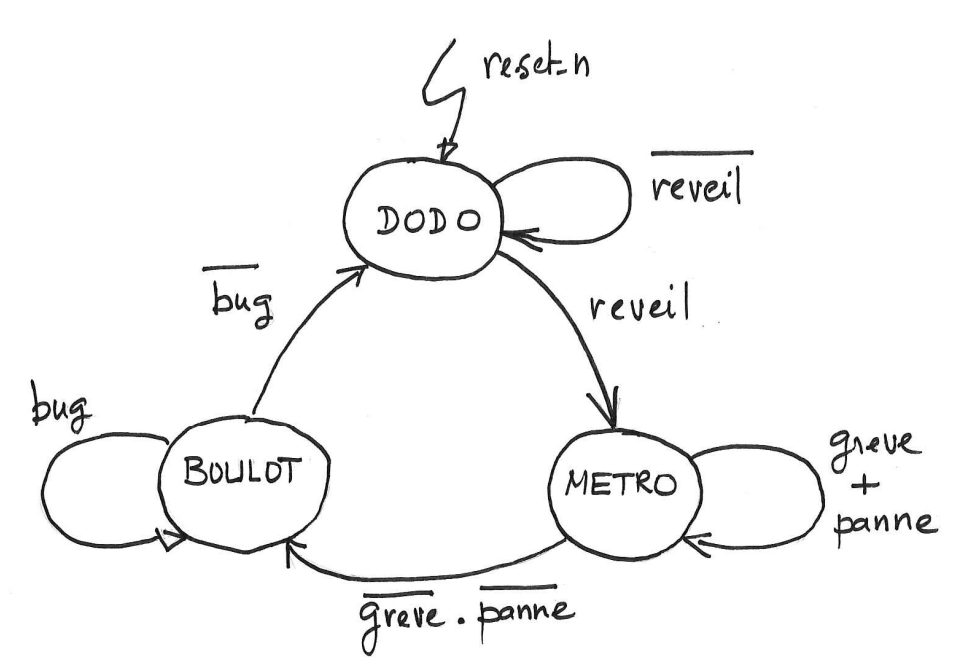
\includegraphics[width=8cm]{./iloveparis.png}
  \caption{Diagramme états-transitions de l'automate "I love Paris"}
  \label{iloveparis}
\end{figure}



\boxed{Questions}
\begin{enumerate}
  \item Vérifier que les équations d'état suivant sont bien données par, dans le cas d'un encodage one-hot :

  $\left\{
  \begin{array}{rl}
    Q_0 &= D_0.\overline{reveil}+D_2.\overline{bug} \\
    Q_1 &= D_0.reveil+D_1.(greve+panne)\\
    Q_2 &= D_1.\overline{greve}.\overline{panne}+D_2.bug\\
  \end{array}
  \right.$

  \item Coder l'automate "I\_love\_Paris" en VHDL, au niveau logique, en prenant soin de bien coder les bascules D à l'aide de processus.
  \lstinputlisting[language=VHDL]{./code/i_love_paris_logic.vhd}

  \item Ajouter un signal de sortie à votre convenance.\footnote{Sans signal de sortie, les synthétiseurs considèrent que la meilleure optimisation
  consiste --à raison-- à générer un circuit absolument vide !}
  \item Utilisez le testbench donné sous Moodle pour tester votre automate. Observez le résultat.
\end{enumerate}

\section{Descriptions d'automates au niveau RTL}


\boxed{Questions}
\begin{enumerate}
  \item Coder l'automate "I\_love\_Paris" en VHDL, au niveau RTL, en vous inspirant de l'exemple donné.
\end{enumerate}

\lstinputlisting[language=VHDL]{./code/i_love_paris.vhd}


\paragraph{Remarques}
Notez que si la version RTL est plus longue, elle est plus explicite.

\end{document}
